\documentclass[notes,11pt, aspectratio=169]{beamer}

\usepackage{pgfpages}
% These slides also contain speaker notes. You can print just the slides,
% just the notes, or both, depending on the setting below. Comment out the want
% you want.
\setbeameroption{hide notes} % Only slide
%\setbeameroption{show only notes} % Only notes
%\setbeameroption{show notes on second screen=right} % Both

\usepackage{helvet}
\usepackage[default]{lato}
\usepackage{array}

\usepackage[backend=biber,style=authoryear,
sorting=ynt,citestyle=authoryear]{biblatex}
\addbibresource{Paper/papercitations.bib}

\usepackage{tikz}
\usepackage{verbatim}
\setbeamertemplate{note page}{\pagecolor{yellow!5}\insertnote}
\usetikzlibrary{positioning}
\usetikzlibrary{snakes}
\usetikzlibrary{calc}
\usetikzlibrary{arrows}
\usetikzlibrary{decorations.markings}
\usetikzlibrary{shapes.misc}
\usetikzlibrary{matrix,shapes,arrows,fit,tikzmark}
\usepackage{amsmath}
\usepackage{mathpazo}
\usepackage{hyperref}
\usepackage{lipsum}
\usepackage{multimedia}
\usepackage{graphicx}
\usepackage{multirow}
\usepackage{graphicx}
\usepackage{dcolumn}
\usepackage{bbm}
\newcolumntype{d}[0]{D{.}{.}{5}}
\usepackage{subfigure}
\usepackage{import}
\usepackage{fontawesome5}

\usepackage{changepage}
\usepackage{appendixnumberbeamer}
\newcommand{\beginbackup}{
   \newcounter{framenumbervorappendix}
   \setcounter{framenumbervorappendix}{\value{framenumber}}
   \setbeamertemplate{footline}
   {
     \leavevmode%
     \hline
     box{%
       \begin{beamercolorbox}[wd=\paperwidth,ht=2.25ex,dp=1ex,right]{footlinecolor}%
%         \insertframenumber  \hspace*{2ex} 
       \end{beamercolorbox}}%
     \vskip0pt%
   }
 }
\newcommand{\backupend}{
   \addtocounter{framenumbervorappendix}{-\value{framenumber}}
   \addtocounter{framenumber}{\value{framenumbervorappendix}} 
}

\setbeamertemplate{blocks}[rounded]
\setbeamercolor{block title}{bg=eggplant!70, fg=white}
\setbeamercolor{block body}{bg=eggplant!30}

\usepackage{graphicx}
\usepackage[space]{grffile}
\usepackage{booktabs}

% These are my colors -- there are many like them, but these ones are mine.
\definecolor{sage}{RGB}{102,153,102}
\definecolor{cambridgeblue}{RGB}{104, 166, 145}
\definecolor{yellow}{RGB}{255,173,1}
\definecolor{purple}{RGB}{153,102,153}
\definecolor{ashgray}{RGB}{191, 211, 193}
\definecolor{eggplant}{RGB}{105, 79, 93}
\definecolor{silver}{RGB}{192, 197, 193}
\definecolor{darkcyan}{RGB}{78, 135, 140}
\definecolor{lightcyan}{RGB}{201, 228, 231}
\definecolor{columbiablue}{RGB}{187, 213, 237}
\definecolor{lightblue}{RGB}{184, 219, 217}
\definecolor{earthyellow}{RGB}{234, 180, 100}

\setbeamercolor{mycolor}{fg=white,bg=sage}

% colors for diagrams
\definecolor{diagramtan}{RGB}{225,190,106}
\definecolor{diagramteal}{RGB}{64, 176, 166}
\definecolor{diagrampurple}{RGB}{170, 131, 239}
\definecolor{diagramred}{RGB}{146, 79, 79}


\hypersetup{
  colorlinks=false,
  linkbordercolor = {white},
  linkcolor = {sage}
}

\newcommand{\btVFill}{\vskip0pt plus 1filll}


%% I use a beige off white for my background
\definecolor{MyBackground}{RGB}{255,253,218}

%% Uncomment this if you want to change the background color to something else
%\setbeamercolor{background canvas}{bg=MyBackground}

%% Change the bg color to adjust your transition slide background color!
\newenvironment{transitionframe}{
  \setbeamercolor{background canvas}{bg=lightcyan}
  \begin{frame}[plain,noframenumbering]}{
    \end{frame}
}

\setbeamercolor{frametitle}{fg=black, bg=lightcyan}
\setbeamercolor{title}{fg=black}
\setbeamertemplate{footline}{%
  \raisebox{5pt}{\makebox[\paperwidth]{\hfill\makebox[15pt]{\scriptsize\insertframenumber}}}}
\setbeamertemplate{navigation symbols}{} 
\setbeamertemplate{itemize items}{$\bullet$}
\setbeamercolor{itemize item}{fg=lightcyan}
\setbeamercolor{itemize subitem}{fg=lightcyan}
\setbeamercolor{enumerate item}{fg=black}
\setbeamercolor{enumerate subitem}{fg=black}
\setbeamercolor{button}{bg=eggplant!80,fg=white}

\setbeamertemplate{frametitle}
{
    \nointerlineskip
    \begin{beamercolorbox}[sep=0.3cm,ht=2em,wd=\paperwidth]{frametitle}
        \vbox{}\vskip-2ex%
        \strut\insertframetitle\strut
        \vskip-0.8ex%
    \end{beamercolorbox}
}



% If you like road maps, rather than having clutter at the top, have a roadmap show up at the end of each section 
% (and after your introduction)
% Uncomment this is if you want the roadmap!
% \AtBeginSection[]
% {
%    \begin{frame}
%        \frametitle{Roadmap of Talk}
%        \tableofcontents[currentsection]
%    \end{frame}
% }

\setbeamercolor{section in toc}{fg=sage}
\setbeamercolor{subsection in toc}{fg=sage}
\setbeamersize{text margin left=1em,text margin right=1em} 

\newenvironment{wideitemize}{\itemize\addtolength{\itemsep}{10pt}}{\enditemize}

\usepackage{environ}
\NewEnviron{videoframe}[1]{
  \begin{frame}
    \vspace{-8pt}
    \begin{columns}[onlytextwidth, T] % align columns
      \begin{column}{.58\textwidth}
        \begin{minipage}[t][\textheight][t]
          {\dimexpr\textwidth}
          \vspace{8pt}
          \hspace{4pt} {\Large \sc \textcolor{blue}{#1}}
          \vspace{8pt}
          
          \BODY
        \end{minipage}
      \end{column}%
      \hfill%
      \begin{column}{.42\textwidth}
        \colorbox{green!20}{\begin{minipage}[t][1.2\textheight][t]
            {\dimexpr\textwidth}
            Face goes here
          \end{minipage}}
      \end{column}%
    \end{columns}
  \end{frame}
}

\title[]{\textcolor{sage}{Does Hospital Leadership Matter? \newline
Evidence from Pay-for-Performance}}

\author[]{Hanna Glenn}
\date{}


\begin{document}

%%% TIKZ STUFF
\tikzset{   
        every picture/.style={remember picture,baseline},
        every node/.style={anchor=base,align=center,outer sep=1.5pt},
        every path/.style={thick},
        }
\newcommand\marktopleft[1]{%
    \tikz[overlay,remember picture] 
        \node (marker-#1-a) at (-.3em,.3em) {};%
}
\newcommand\markbottomright[2]{%
    \tikz[overlay,remember picture] 
        \node (marker-#1-b) at (0em,0em) {};%
}
\tikzstyle{every picture}+=[remember picture] 
\tikzstyle{mybox} =[draw=black, very thick, rectangle, inner sep=10pt, inner ysep=20pt]
\tikzstyle{fancytitle} =[draw=black,fill=red, text=white]
%%%% END TIKZ STUFF

% Title Slide
\begin{frame}[plain]
% Background image
\begin{tikzpicture}[remember picture,overlay]
    \node
[
    above=0.5cm,
    align=center,
    fill=lightcyan,
    rounded corners,
    inner xsep=15pt,
    inner ysep=10pt, 
    minimum width=0.9\textwidth,
    text width=0.6\textwidth
] (title) at (current page.center)
{
    \LARGE Does Hospital Leadership Matter?  \\[5pt]
    \large Evidence from Pay-for-Performance
};
% Author 
\node[below=1cm] (author) at (title.south){\large Hanna Glenn, Emory University};
% Date
\node[below=0.25cm] (date) at (author.south){\today};
\end{tikzpicture}
    
\end{frame}

\section{Intro}

\begin{frame}{Leadership Matters}
\centering
    \begin{tikzpicture}
        % First image (top-left)
        \node[anchor=north west] (img1) at (0, 3) {
\includegraphics[width=0.75\textwidth]{Graphics/theroleleadershiphasincompanyculture.png}};
        \draw[line width=.45mm, lightcyan] (img1.north west) rectangle (img1.south east);
        
        % Second image (slightly down and right of the first image)
        \node[anchor=north west] (img2) at (0, -.25) {
\includegraphics[width=0.75\textwidth]{Graphics/linkingbusinessstrategyandleadershipforbetteroutcomes.png}};
        \draw[line width=.45mm, lightcyan] (img2.north west) rectangle (img2.south east);
    
        
        % Fourth image (bottom-right)
        %\node[anchor=north west] (img4) at (0, -2) {
\includegraphics[width=0.55\textwidth]{Graphics/theroleofleadershipinorganizationalsuccess.png}};
        %\draw[line width=.45mm, lightcyan] (img4.north west) rectangle (img4.south east);


    \end{tikzpicture}
\end{frame}

\begin{frame}{Leadership Characteristics and Firm Behavior/Performance}

\large

\textbf{Gender}
\begin{itemize}
    \item \normalsize Female board members $\implies$ lower firm value, less employment reduction \\ \scriptsize(\cite{ahern2012changing}; \cite{matsa2013female}) \normalsize
    \item Female executives $\implies$ female wage distribution \scriptsize (\cite{flabbi2019female}) \normalsize
\end{itemize}

\vspace{4mm}

\textbf{Prior Experience}
\begin{itemize}
    \item \normalsize General background CEOs paid more \scriptsize (\cite{custodio2013generalists}) \normalsize
    \item Background matters for acquisitions \scriptsize(\cite{custodio2013ceos}) \normalsize

\vspace{1mm}
    
    \item Military experience CEOs \scriptsize (\cite{benmelech2015military})
\end{itemize}

\vspace{4mm}

\textbf{Age}
\begin{itemize}
    \item \normalsize Young male CEOs more aggressive in M\&A \scriptsize (\cite{levi2010deal})
\end{itemize}


\end{frame}

\begin{frame}{Gaps in Literature}
    \large
    \begin{enumerate}
        \item Findings are limited to large, publicly traded firms

\vspace{2mm}
        
        \begin{itemize}
            \item \normalsize Different objectives/incentives in other types of firms (nonprofits)
        \end{itemize}

        \vspace{10mm}
        
        \item Unclear whether leadership matters when policies change incentives
    \end{enumerate}
\end{frame}


\begin{frame}{Addressing the Gaps}

    \Large
    \begin{block}{}
    \begin{center}
    I examine the role of leadership in nonprofit hospitals
    
    responding to policy incentives
    \end{center}
    \end{block}


\vspace{5mm} \large \pause

\begin{enumerate}
    \item \textbf{Hospital care makes up a third of health care spending} \scriptsize (\cite{cms2024nhe}) \normalsize

\vspace{2mm}
    
    \begin{itemize}
        \item \normalsize Nonprofits drive the hospital industry \scriptsize (\cite{ASPE_2023}) \normalsize
    \end{itemize}

\vspace{8mm}

    \item \large \textbf{Policies often aim to improve the value of health care delivery}

\vspace{2mm}

    \begin{wideitemize}
        \item \normalsize Unclear how leaders interact with this goal
    \end{wideitemize}

    \end{enumerate}
\end{frame}

\begin{frame}{Research Question}
    \centering
    \Large
    Do executives with clinical training 

    \vspace{1mm}
    
    affect response to pay-for-performance incentives 

    \vspace{1mm}
    
    of nonprofit hospitals in the US?
\end{frame}

\begin{frame}{Why Clinical Training?}

\large

\textbf{Do physicians make good firm leaders?}

\vspace{2mm}

\begin{wideitemize}
    \item Relevant expertise \scriptsize (\cite{Stajduhar_2023}, \cite{Ahmed_2022}) \large

    
    \item Lack of business training \scriptsize (\cite{HarvardBusinessReview2018})
\end{wideitemize}

\vspace{12mm}

\textbf{Potentially correlated with how the leader values quality versus profit}
\end{frame}

\begin{frame}{Pay-for-Performance Incentives}
    \large
    \begin{block}{\Large Main Takeaway:}
        \large 
        \centering
        \vspace{1mm}
        Hospitals now have financial incentives to improve quality

        \vspace{1mm}
    \end{block}

    \vspace{6mm}
    
    \textbf{Quality: 30-day readmissions \& 30-day mortality}

    \vspace{5mm}

    Hospital Readmissions Reduction Program
    \begin{itemize}
        \item Penalized high readmissions
        \item Pneumonia, Heart Attack (AMI), Heart Failure
    \end{itemize}

    \vspace{5mm}

    Hospital Value-Based Purchasing Program
    \begin{itemize}
        \item Score metric determines rewards
        \item Rewards high metric
    \end{itemize}
\end{frame}

\begin{frame}{Preview of Main Findings}

\large

\textbf{Non-clinical executive teams respond more to financial incentives on quality}

\vspace{3mm}

\begin{wideitemize}
    \item Through readmission rates
    \item Non-clinical executive teams behave like profit-driven hospitals
\end{wideitemize}
\end{frame}

\begin{frame}{Contribution}
\large
    \textbf{Hospital Executives/Board of Directors}

\vspace{2mm}
    
    \begin{wideitemize}
        \item \normalsize Physician board members $\implies$ lower public donations \scriptsize (\cite{brickley2010board}) \normalsize
        \item No correlation b/w CEOs and hospital productivity in England \scriptsize (\cite{janke2019impact})\normalsize
        \item Public hospitals in Chile improved when older physicians left CEO \scriptsize (\cite{otero2022managers}) \normalsize
    \end{wideitemize}

    \vspace{5mm}\pause

    \textbf{Hospital Response to Pay-for-Performance}

\vspace{2mm}
    
    \begin{wideitemize}
        \item \normalsize Hospitals decreased readmissions \scriptsize (\cite{gupta2021impacts}) \normalsize
        \item Market concentration and systems affect response \scriptsize (\cite{kunz2024assessing}) \normalsize
        \item Rewards had little impact on quality \scriptsize (\cite{norton2018moneyball}; \cite{friedson2019so})
    \end{wideitemize}
\end{frame}

\begin{frame}{Rest of Talk}

\large

    Setting and Data Collection

    \vspace{5mm}

    About Executive Teams

    \vspace{5mm}

    Theoretical Motivation

    \vspace{5mm}

    Effect of Clinical Leadership

    \vspace{5mm}

    Comparison to For-Profits

    \vspace{5mm}

    Signaling vs. Managing
\end{frame}



\section{Setting and Data Collection}

\begin{transitionframe}
\centering \LARGE
    \textcolor{black}{Setting and Data Collection}
\end{transitionframe}

\begin{frame}{About the Executives}\label{nonprofithospexec}

\large
\textbf{What do they do?}

\vspace{2mm}

\begin{wideitemize}
    \item Board of directors selects executives
    \item Executives handle the day-to-day operations of the hospital 
    \item Quality often improved from the top down \scriptsize (\cite{silow2011reducing})
\end{wideitemize}

\vspace{4mm} \pause 

\textbf{Executive teams}

\vspace{2mm}

\begin{wideitemize}
    \item Lot of variation in team organization
    \item CEO and CFO
    \item I focus on the team as a whole instead of specific executive roles
\end{wideitemize}

\btVFill

\hyperlink{executivejob}{\beamergotobutton{executive job}} 

\end{frame}

\begin{frame}{}
    \begin{tikzpicture}
        % First image in the top-left
        \node[anchor=north west] at (0, 4) {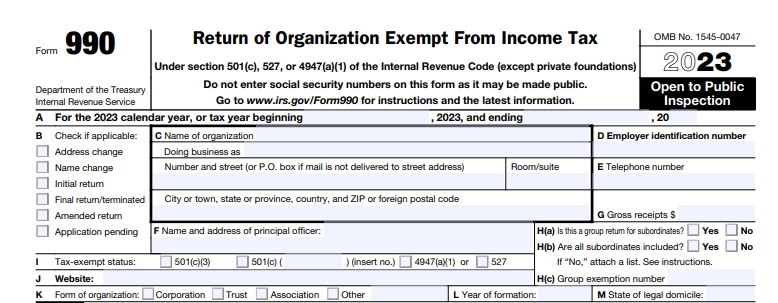
\includegraphics[width=0.7\textwidth]{Graphics/990_snip_frontpage.PNG}};
        % Second image in the middle
        \node[anchor=north west] (img2) at (2.5, 1.5) {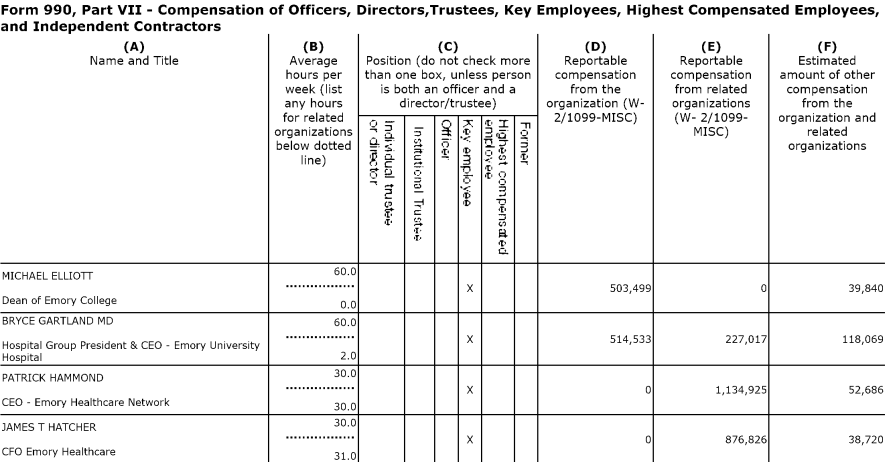
\includegraphics[width=0.75\textwidth]{Graphics/Screenshot 2024-10-03 160258.png}};
        \draw[line width=1mm, eggplant] (img2.north west) rectangle (img2.south east);
    \end{tikzpicture}
\end{frame}

\begin{frame}{Data Collection Process}
\begin{center}
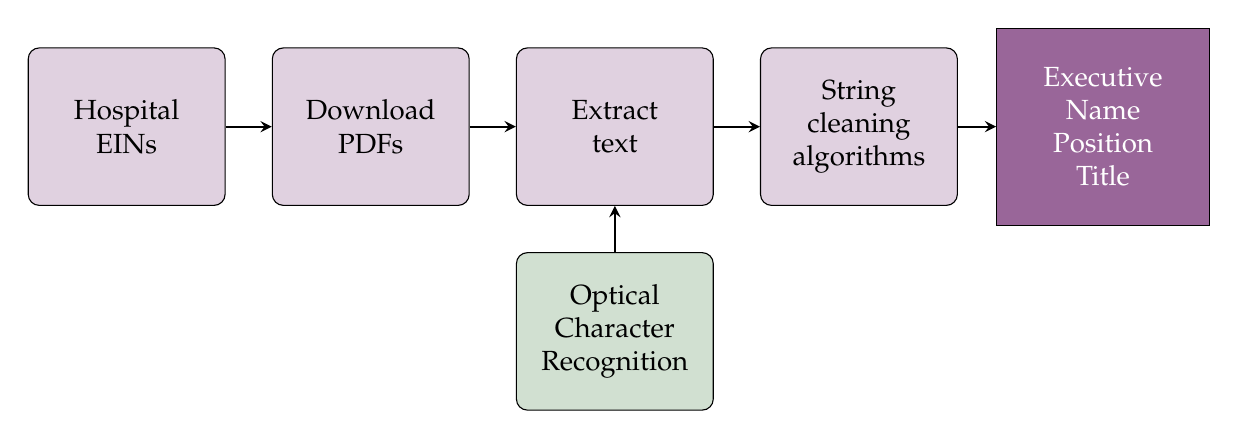
\begin{tikzpicture}[
    node distance=3.1cm and 1.8cm,
    every node/.style={align=center, font=\normalsize},
    process/.style={rectangle, draw, rounded corners, text centered, minimum width=2.5cm, minimum height=2cm, fill=purple!30},
    output/.style={rectangle, draw, text centered, minimum width=2.7cm, minimum height=2.5cm, fill=purple},
    extract/.style={rectangle, draw, rounded corners, text centered, minimum width=2.5cm, minimum height=2cm, fill=sage!30},
    arrow/.style={thick, ->, >=stealth}
]

% Nodes
\node (step1) [process] {Hospital \\EINs};\pause
\node (step2) [process, right of=step1] {Download \\PDFs};
\draw[arrow] (step1) -- (step2); \pause
\node (step3) [process, right of=step2] {Extract\\text};
\draw[arrow] (step2) -- (step3); 
% New green box below step3
\node (extract) [extract, below of=step3, yshift=0.5cm] {Optical\\Character\\Recognition}; 
\draw[arrow] (extract) -- (step3);\pause
\node (step4) [process, right of=step3] {String\\cleaning\\algorithms};
\draw[arrow] (step3) -- (step4); \pause
\node (output) [output, right of=step4, text=white] {Executive\\Name\\Position\\Title};
\draw[arrow] (step4) -- (output);
\end{tikzpicture}
\end{center}
\end{frame}


\begin{frame}{Merge to Other Data}

\large
    \textbf{Hospital:} 

    \vspace{2mm}
    \begin{wideitemize}
        \item AHA
        \item Hospital Compare
        \item CMS Case Mix Index
        \item Health Care Cost Report Information System (HCRIS)
    \end{wideitemize}

    \vspace{7mm}

    \textbf{Physician:} 

    \vspace{2mm}

    \begin{itemize}
        \item Manually match physician executives to NPPES NPI number
    \end{itemize}
\end{frame}


\section{About Executive Teams}

\begin{transitionframe}
\centering \LARGE
    \textcolor{black}{Descriptive Statistics}
\end{transitionframe}

\begin{frame}{Executive Teams}
\begin{table}[ht!]
\centering
\begin{tabular}[t]{lccc}
\toprule
 & Ever & Always & Never\\
  & Clinical Exec & Clinical Exec & Clinical Exec\\
\midrule
\addlinespace[0.3em]
Number Executives & 4.82 & 5.19 & 2.86\\
Fraction Clinical Execs & 0.20 & 0.26 & 0.00\\
Fraction Int. Medicine Execs & 0.06 & 0.08 & 0.00\\
Has a CMO & 0.55 & 0.52 & 0.07\\
Has Clinical CEO & 0.25 & 0.10 & 0.00\\
\addlinespace[0.6em]
Num. Hospitals & 452 & 62 & 385\\
\bottomrule
\end{tabular}
\end{table}
\end{frame}

\begin{frame}{Doctors on Executive Teams (N=941)}
\begin{table}[ht!]
\centering
\begin{tabular}[t]{lc}
\toprule
& Mean\\
\midrule
Age & 52.56\\
Female & 0.11\\
CEO & 0.15\\
CMO & 0.36\\
CQO & 0.09\\
\addlinespace[0.3em]
\multicolumn{2}{l}{\textbf{Specialty}}\\
\hspace{1em}Internal Medicine & 0.32\\
\hspace{1em}Family Medicine & 0.18\\
\hspace{1em}Surgery & 0.14\\
\hspace{1em}Emergency Medicine \hspace{4mm} & 0.11\\
\hspace{1em}Pediatrics & 0.06\\
\hspace{1em}Other & 0.16\\
\bottomrule
\end{tabular}
\end{table}
\end{frame}


\begin{frame}{Hospital Statistics}\label{sumstats}
\vspace{-3mm}
\begin{table}[ht!]
\centering
\begin{tabular}[t]{lccc}
 & Ever & Always & Never\\
  & Clinical Exec &Clinical Exec &Clinical Exec\\
\midrule
\addlinespace[0.3em]
\multicolumn{4}{l}{\textbf{Hospital Characteristics}}\\
\hspace{1em}Academic Med. Center & 0.41 & 0.51 & 0.20\\
\hspace{1em}Number Beds & 227 & 218 & 102\\
\hspace{1em}Physician Owned & 0.01 & 0.02 & 0.02\\
\hspace{1em}System Affiliated & 0.57 & 0.56 & 0.42\\
\addlinespace[0.3em]
\multicolumn{4}{l}{\textbf{Penalty/Payment Variables}}\\
\hspace{1em}Ever Received HVBP Incentive & 0.79 & 0.77 & 0.59\\
\hspace{1em}Penalized for one condition & 0.19 & 0.25 & 0.13\\
\hspace{1em}Penalized for AMI + HF & 0.07 & 0.05 & 0.03\\
\hspace{1em}Penalized for AMI + Pneumonia & 0.02 & 0.02 & 0.02\\
\hspace{1em}Penalized for HF + Pneumonia & 0.41 & 0.40 & 0.33\\
\hspace{1em}Penalized for All Conditions & 0.31 & 0.31 & 0.20\\
\bottomrule
\end{tabular}
\end{table}
\hyperlink{forprofitstats}{\beamergotobutton{for-profit stats}}
\end{frame}

\begin{frame}{Raw Outcomes, controlling for baseline case mix index}\label{outcomes}
\begin{center}
    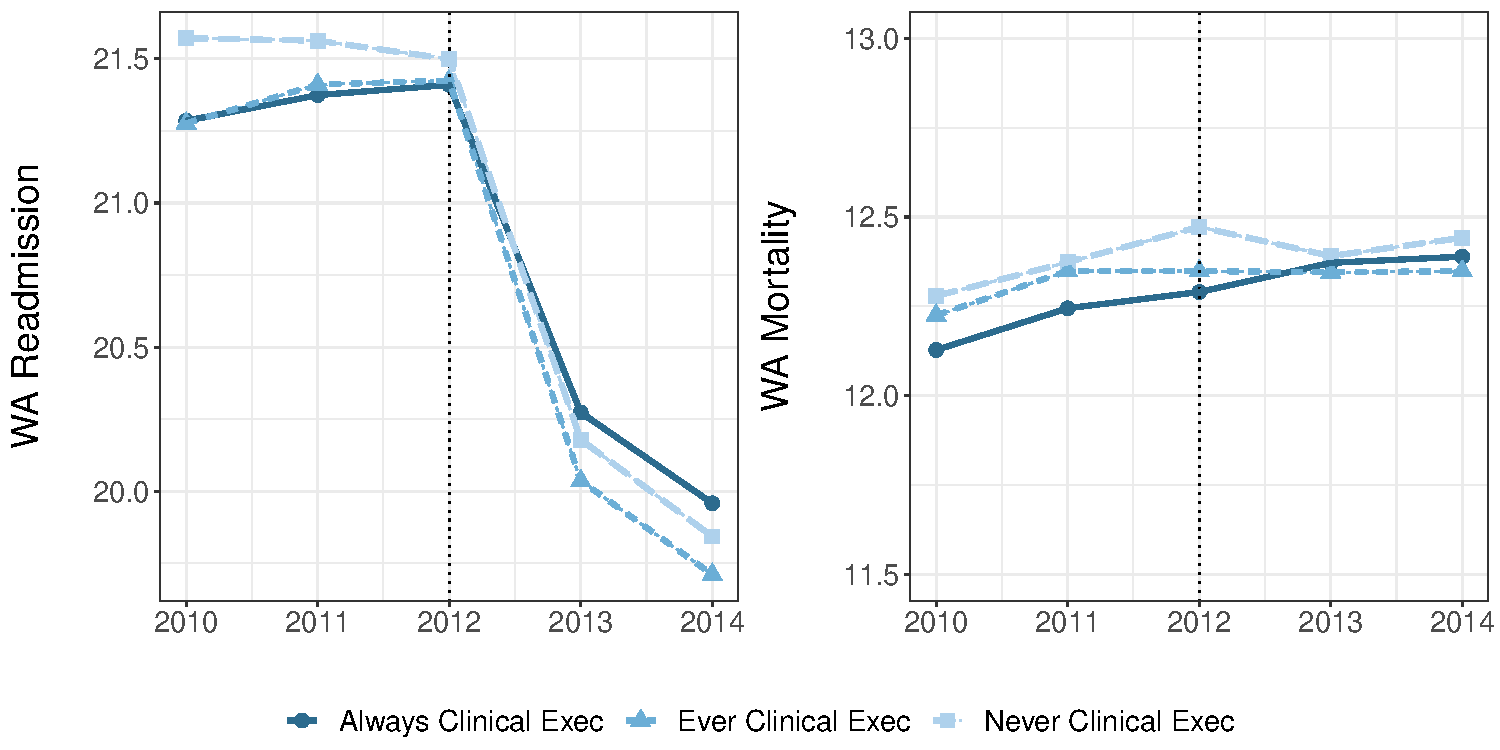
\includegraphics[width=.92\textwidth]{Objects/outcomes_graph_presentation.pdf}
\end{center}
    \btVFill
    \hyperlink{fp_outcomes}{\beamergotobutton{with for-profit}}
\end{frame}

\section{Theoretical Framework}

\begin{transitionframe}
\centering \LARGE
    \textcolor{black}{Theoretical Framework}
\end{transitionframe}

\begin{frame}{Hospital Objectives: Profit versus Patient Welfare}
    \Large
    \centering
    \begin{equation*}
        \max_{\theta}\hspace{2mm} \alpha\pi(\theta) + (1-\alpha)u(\theta)
    \end{equation*}
\end{frame}

\begin{frame}[noframenumbering]{Hospital Objectives: Profit versus Patient Welfare} \Large
    \begin{equation*}
\max_{\theta}\hspace{2mm}\alpha
\tikz[baseline]{
    \node[draw=sage,rounded corners,anchor=base] (m1)
    {$\pi(\theta)$};
    \node[above of=m1, text=sage, yshift=5mm] (l1) {profit};
    \draw[-,sage] (l1) -- (m1);
}
+ (1-\alpha)\hspace{-11mm}
\tikz[baseline]{
    \node[draw=sage,rounded corners,anchor=base] (m2)
    {$u(\theta)$};
    \node[above of=m2, text=sage, yshift=5mm] (l2) {patient welfare};
    \draw[-,sage] (l2) -- (m2);
}
\end{equation*}
\end{frame}

\begin{frame}[noframenumbering]{Hospital Objectives: Profit versus Patient Welfare} \Large
    \begin{equation*}
\max_{\theta}\hspace{2mm}\alpha\pi(\hspace{-5mm}
\tikz[baseline]{
    \node[draw=purple,rounded corners,anchor=base] (m1)
    {$\theta$};
    \node[above of=m1, text=purple, yshift=5mm] (l1) {quality};
    \draw[-,purple] (l1) -- (m1);
}
\hspace{-5mm}) + (1-\alpha)u(\hspace{-5mm}
\tikz[baseline]{
    \node[draw=purple,rounded corners,anchor=base] (m2)
    {$\theta$};
    \node[above of=m2, text=purple, yshift=5mm] (l2) {quality};
    \draw[-,purple] (l2) -- (m2);
}
\hspace{-5mm})
\end{equation*}
\end{frame}

\begin{frame}[noframenumbering]{Hospital Objectives: Profit versus Patient Welfare} \Large
    \begin{equation*}
\max_{\theta}\hspace{-4mm}
\tikz[baseline]{
    \node[draw=earthyellow,rounded corners,anchor=base] (m1)
    {$\alpha$};
    \node[above of=m1, text=earthyellow, yshift=5mm] (l1) {weight on\\profit};
    \draw[-,earthyellow] (l1) -- (m1);
}
\hspace{-8mm}\pi(\theta) + \hspace{-7mm}
\tikz[baseline]{
    \node[draw=earthyellow,rounded corners,anchor=base] (m2)
    {$(1-\alpha)$};
    \node[above of=m2, text=earthyellow, yshift=5mm] (l2) {weight on\\patient welfare};
    \draw[-,earthyellow] (l2) -- (m2);
}
\hspace{-7mm}u(\theta)
\end{equation*}
\end{frame}


\begin{frame}{Choice of Quality}\label{choiceofquality}

\vspace{9mm}

\Large

    \begin{columns}
    \begin{column}{0.5\textwidth}
    \begin{center}
        \underline{Fee-for-Service}

        \vspace{3mm}

            $\pi$ $\downarrow$ in $\theta$
    \end{center}
    \end{column}
    \begin{column}{0.5\textwidth}  %%<--- here
    \begin{center}
        \underline{Pay-for-Performance}

        \vspace{3mm}


            $\pi$ $\uparrow$ in $\theta$
    \end{center}
    \end{column}
\end{columns}

\btVFill

\begin{block}{\Large Fee-for-service to Pay-for-performance}
    \centering
    \vspace{3mm}
    Higher $\alpha$ $\implies$ larger response

    \vspace{3mm}
\end{block}

\hyperlink{choiceofqualityapp}{\beamergotobutton{more details}}
\end{frame}

\begin{frame}{Informing the Empirical Analysis}

\large
    \begin{enumerate}
        \item If clinicians affect $\alpha$, they affect quality change after P4P

        \vspace{8mm}\pause
        \item If non-clinicians have higher $\alpha$, they act more like for-profits

        \vspace{8mm}\pause
        \item Mechanism could be revealing objectives or changing objectives
    \end{enumerate}
\end{frame}


\section{Effect of Clinical Leadership on Response}

\begin{transitionframe}
\centering \LARGE
    \textcolor{black}{Effect of Clinical Leadership on Response to P4P}
\end{transitionframe}

\begin{frame}{Estimation}\label{est_equation}

\large
    \textbf{Compare always clinical to never clinical hospital executive teams:}

    \vspace{3mm}\large
    \begin{equation*}
    y_{ht} = \beta \text{ (clinical training x post 2012)}_{ht} + \gamma_{h} + \delta_t + \epsilon_{ht}
    \end{equation*}

    \vspace{3mm}
    \begin{wideitemize}
        \item $y_{ht}$: weighted average readmission/ mortality rates
        \item Leverage \textit{timing} of the programs
    \end{wideitemize}

    \vspace{8mm}\pause

    Different methods:
    \begin{itemize}
        \item No weights
        \item \textbf{``Synthetic DiD" type weights} 
        \item Coarsened exact matching 
    \end{itemize}
\end{frame}

\begin{frame}{Identification Assumptions}

\large
\begin{wideitemize}
    \item Parallel trends
    \item No other 2012 event correlated with executive team and outcomes
    \item No hospital characteristics perfectly correlated with executive team
    \item No anticipation of incentive changes
    \item Stability in clinical executives not correlated with incentive change
\end{wideitemize}
\end{frame}

\begin{frame}{Average Team Changes Over Time}
\centering 
    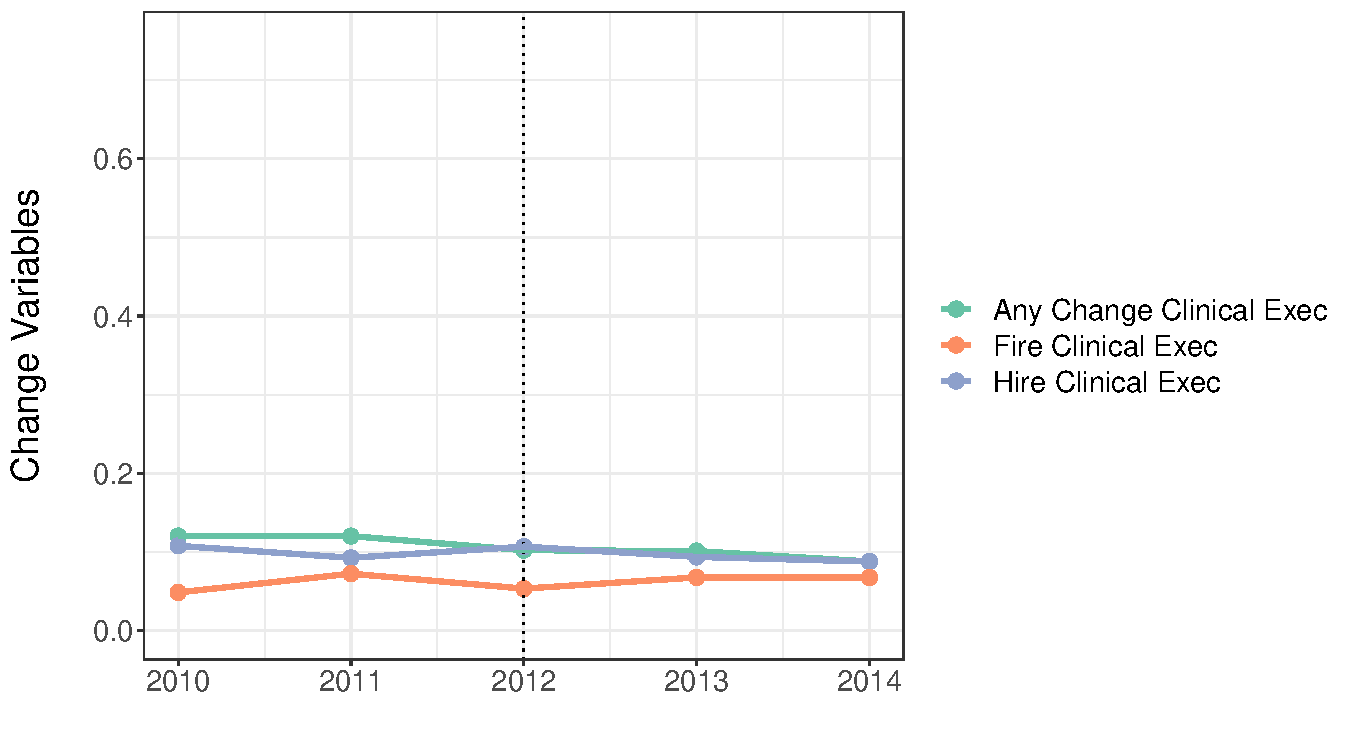
\includegraphics[width=.8\textwidth]{Objects/change_means.pdf}
\end{frame}

\begin{frame}{Changes are not correlated with policy exposure}
\centering \small
\begin{equation*}\label{eq:change2}
    \text{change}_{ht} = \sum_{j=2011}^{2014}\beta_j(\mathbf{1}\{t=j\}\times \text{Program Exposed})_{ht} + \alpha_h + \epsilon_{ht},
    \end{equation*}

    \btVFill

    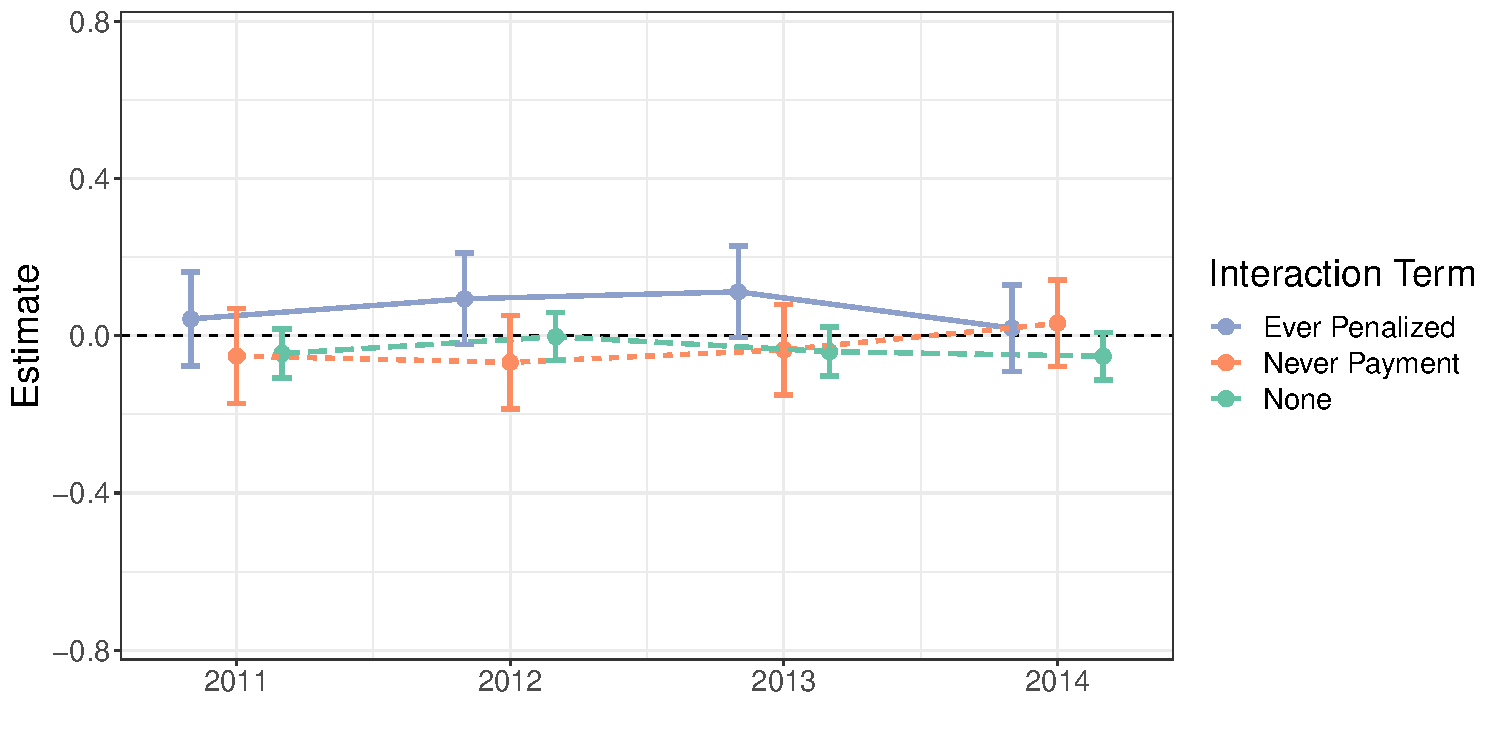
\includegraphics[width=.7\textwidth]{Objects/change_analysis_plot.pdf}
    
\end{frame}

\begin{frame}{Readmission Rates}\label{main:readrates}
\large
    \begin{columns}
    \column{0.5\textwidth}
        \centering
        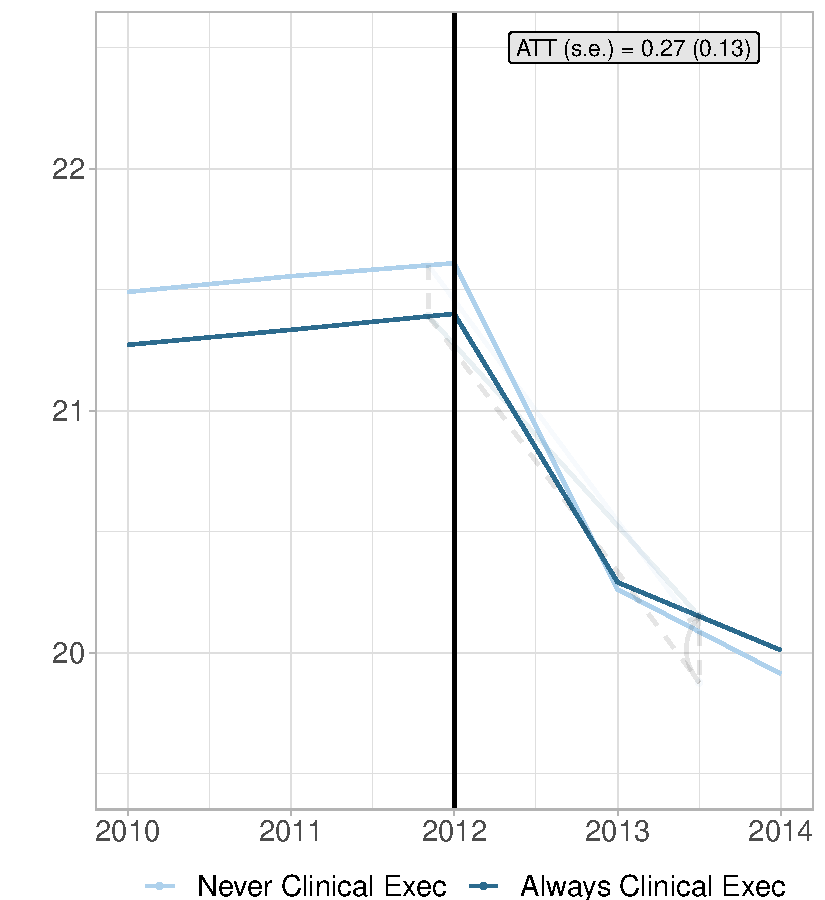
\includegraphics[width=.9\textwidth]{Objects/read_md_nomd_synth_graph.pdf}
    \column{0.5\textwidth}
        \begin{wideitemize}
            \item Magnitude: 0.3ppt difference

\vspace{5mm}
            
            \item Large relative to effect of HRRP (1ppt)
        \end{wideitemize}
        
        \vspace{20mm}

        \hyperlink{int_margin}{\beamergotobutton{intensive margin}}
        \hyperlink{cmi}{\beamergotobutton{due to patient selection?}}
        \hyperlink{specifications}{\beamergotobutton{specifications}}
        \hyperlink{specialty}{\beamergotobutton{specialty}}
        
    \end{columns}
\end{frame}

\begin{frame}{Mortality Rates}
\large
    \begin{columns}
    \column{0.5\textwidth}
        \centering
        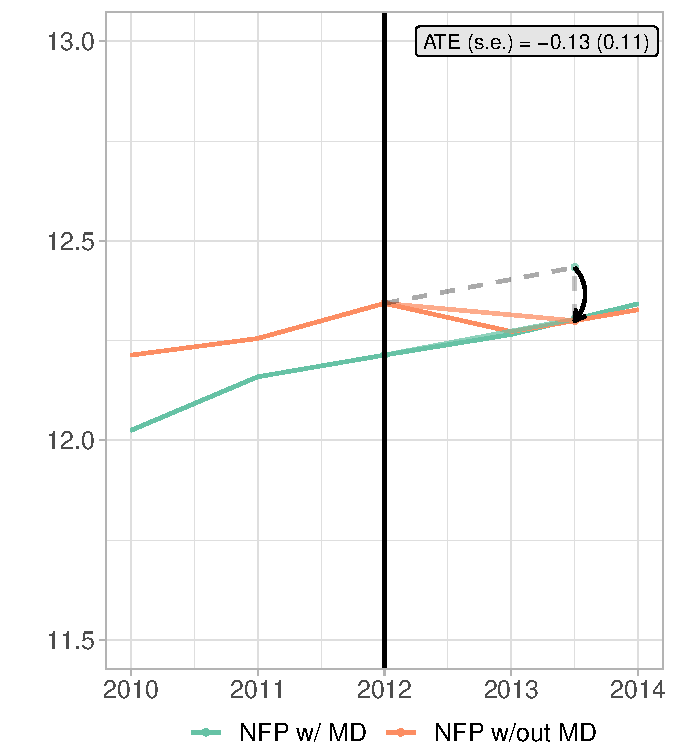
\includegraphics[width=.9\textwidth]{Objects/mort_md_nomd_synth_graph.pdf}
    \column{0.5\textwidth}
        \begin{wideitemize}
            \item Magnitude: 0.1ppt 

            \vspace{5mm}
            
            \item Mortality is noisy measure 
        \end{wideitemize}
    \end{columns}
\end{frame}

\section{Comparison to For-Profit Hospitals}


\begin{transitionframe}
\centering \LARGE
    \textcolor{black}{Comparison to For-Profit Hospitals}
\end{transitionframe}

\begin{frame}{Estimation}
\large
    \textbf{Compare both nonprofit leadership team types to the response of for-profits:}

    \vspace{5mm}\large
    \begin{equation*}
    y_{ht} = \beta \text{ (for-profit x post 2012)}_{ht} + \gamma_{h} + \delta_t + \epsilon_{ht}
    \end{equation*}

    \vspace{10mm}

    Comparison group:
    \begin{itemize}
        \item nonprofit clinical; nonprofit non-clinical
    \end{itemize}

\end{frame}

\begin{frame}{Readmission Rate}
    \begin{columns}
    \column{0.5\textwidth}
        \centering
        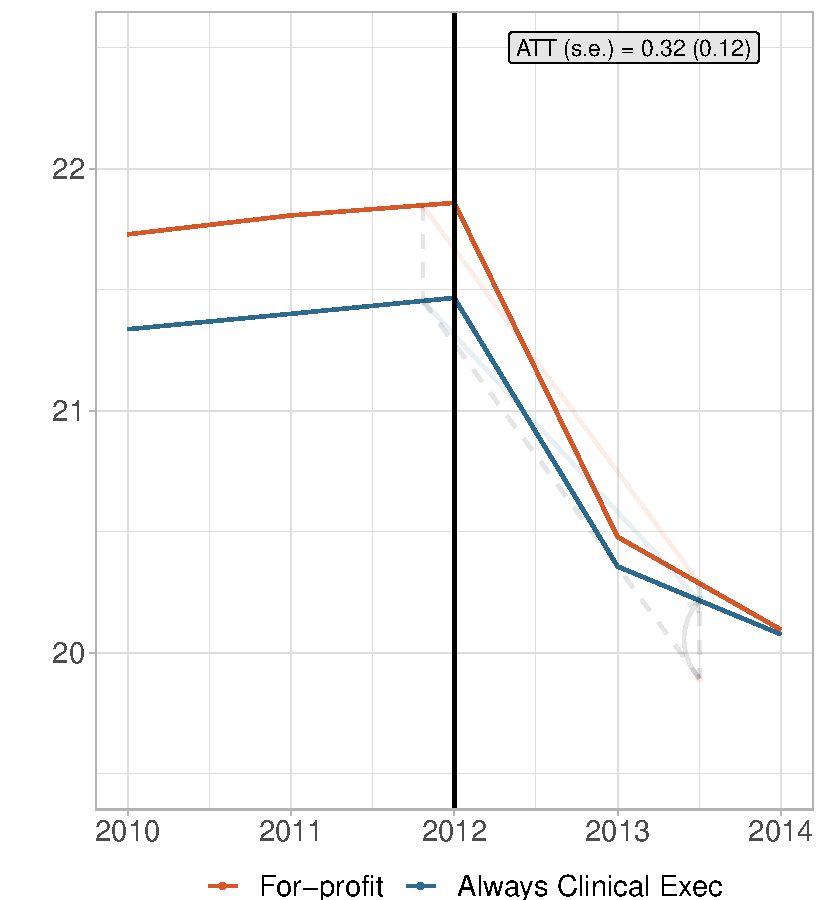
\includegraphics[width=.9\textwidth]{Objects/fp_read_md_synth_graph.pdf}
    \column{0.5\textwidth}
        \centering
        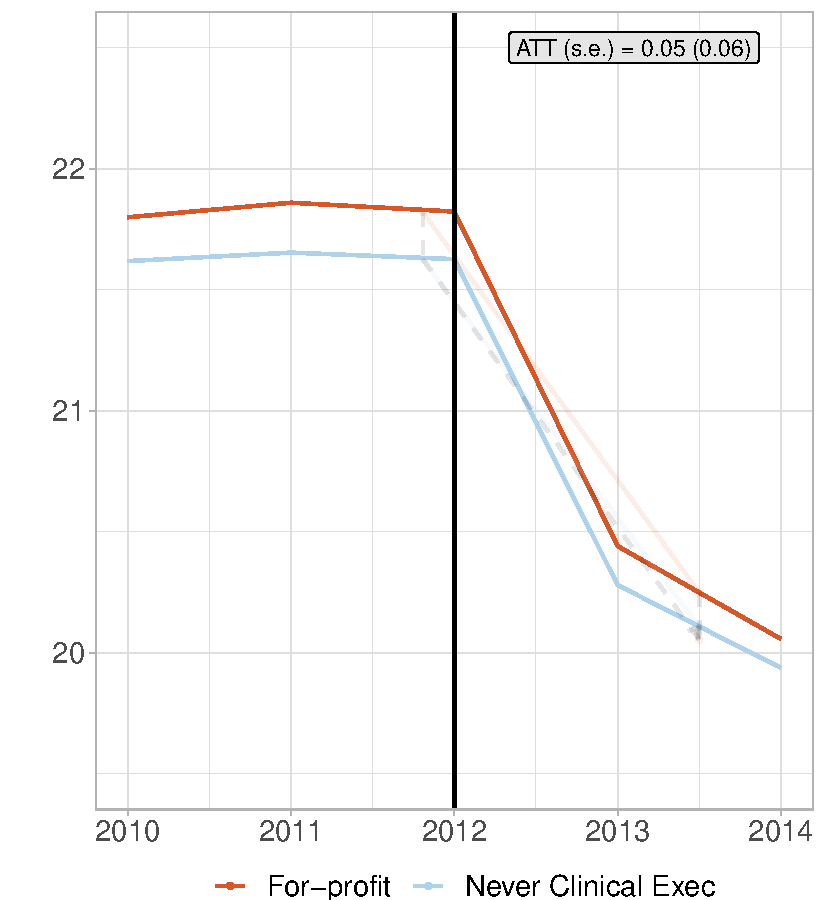
\includegraphics[width=.9\textwidth]{Objects/fp_read_nomd_synth_graph.pdf}
    \end{columns}
\end{frame}

\begin{frame}{Mortality Rate}
    \begin{columns}
    \column{0.5\textwidth}
        \centering
        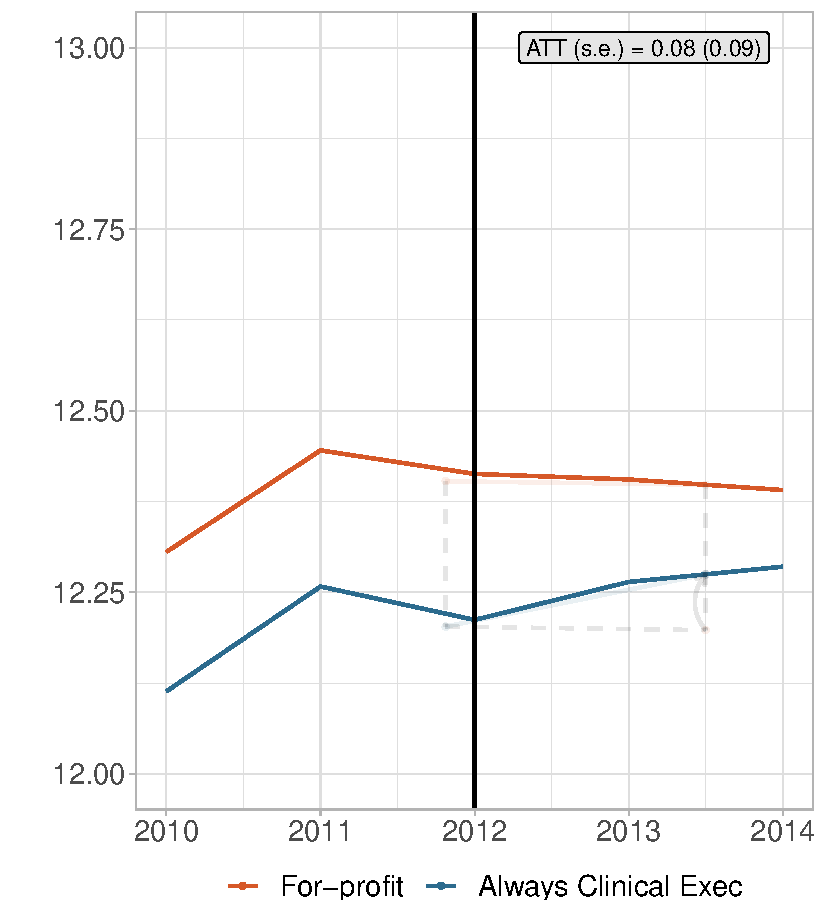
\includegraphics[width=.9\textwidth]{Objects/fp_mort_md_synth_graph.pdf}
    \column{0.5\textwidth}
        \centering
        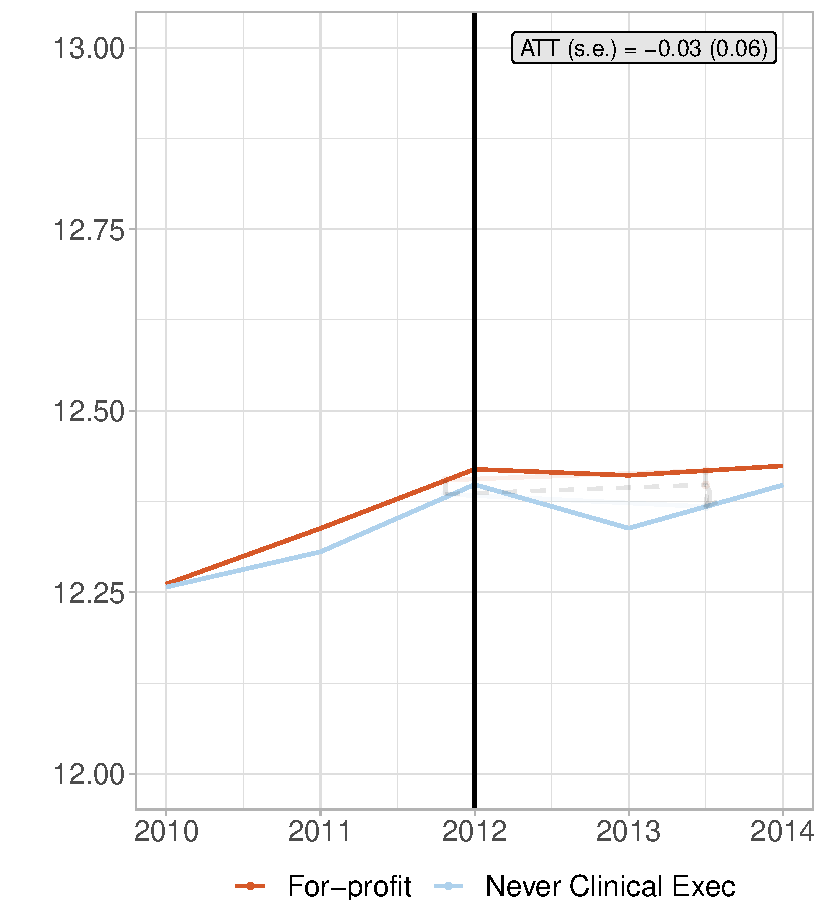
\includegraphics[width=.9\textwidth]{Objects/fp_mort_nomd_synth_graph.pdf}
    \end{columns}
\end{frame}

\section{Signaling vs. Managing}

\begin{transitionframe}
\centering \LARGE
    \textcolor{black}{Signaling vs. Managing}
\end{transitionframe}

\begin{frame}{Hypotheses}

\large
    \textbf{Clinical leaders represent underlying objectives ($\alpha$)}

\vspace{2mm}
    
    \begin{wideitemize}
        \item Timing of the clinical leader doesn't matter 
    \end{wideitemize}

    \vspace{15mm}

    \textbf{Clinical leaders effectively change objectives ($\alpha$)}

\vspace{2mm}
    
    \begin{wideitemize}
        \item Timing of the clinical leader does matter
    \end{wideitemize}
\end{frame}

\begin{frame}{Estimation}
\large
    \begin{figure}[ht!]
\begin{center}
 
 \begin{tabular}{| m{15em} |}
 \hline \vspace{1mm}
 \textbf{Signaling:}\\ [0.5ex]
 \hline\hline 
 \vspace{2mm}
 Treat Group:  \hspace{15mm} Never MD \\
 \vspace{2mm}
 Comparison Group: \hspace{3mm} Ever MD  \\
 [1ex]
 \hline
 \end{tabular}
\hfil   %<---
 \begin{tabular}{|m{18em}|}
 \hline \vspace{1mm}
 \textbf{Managing:}\\ [0.5ex]
 \hline\hline
 \vspace{2mm}
 Treat Group: \hspace{11mm} MD in 2012 \\
 \vspace{2mm}
 Comparison Group:  MD not in 2012  \\
 [1ex]
 \hline
 \end{tabular}
 
\end{center}
 \end{figure}

\end{frame}

\begin{frame}{Results}
    \begin{table}[ht!]
\centering
\begin{tabular}[t]{lcccc}
\toprule
\multicolumn{1}{c}{ } & \multicolumn{2}{c}{\underline{Weighted Avg. Readmission Rate}} & \multicolumn{2}{c}{\underline{Weighted Avg. Mortality Rate}} \\
 & (1) & (2) & (3) & (4)\\
\midrule
Signaling Effect & -0.01 &  & 0.03 & \\
 & (0.07) &  & (0.06) & \\
Managing Effect &  & 0.17 &  & 0.12\\
 &  & (0.1) &  & (0.09)\\
 &  &  &  & \\
Observations & 3,005 & 1,595 & 3,005 & 1,595\\
\bottomrule
\end{tabular}
\end{table}
\end{frame}

\begin{frame}{Summary}
\large
    \textbf{We know very little about whether leaders matter in health care}

    \begin{wideitemize}
        \item This paper: non-clinical executive teams internalize financial incentives more
    \end{wideitemize}

    \vspace{5mm}
    
    \textbf{Implications}
    \begin{itemize}
        \item Not all nonprofits have the same objectives
        \item More clinicians in leadership could shift objectives towards quality
    \end{itemize}

    \vspace{5mm}

    \textbf{Future Work}

    \begin{itemize}
        \item Effects of mandated gender and racial diversity on hospital behavior
        \item Networks of executives over time 
        \item Are leaders correlated with hospital fraudulent behavior?
    \end{itemize}
\end{frame}

\begin{transitionframe}
\centering 
%
\includegraphics[width=.2\textwidth]{Graphics/HannaGlenn_headshot.jpg}

\vspace{5mm}

\Large
    Thank you! 

    \vspace{15mm}
    
    \textcolor{black}{\faEnvelope \hspace{2mm} hanna.glenn@emory.edu}

    \vspace{2mm}
    
    \textcolor{black}{\faTwitter \hspace{2mm} @hannalynnglenn}
\end{transitionframe}




\section{Appendix}

\begin{transitionframe}
\centering \LARGE
    \textcolor{black}{Appendix Slides}
\end{transitionframe}

\appendix

\begin{frame}{Choice of Quality}\label{choiceofqualityapp}
Take FOC, rearrange and take derivative wrt $\alpha$:

\vspace{5mm}

\begin{equation*}
    \frac{du'(\theta)}{d\alpha} = \frac{-1}{(1-\alpha)^2}\pi'(\theta)
\end{equation*}

\vspace{5mm}

$\pi'(\theta)$:

\vspace{3mm}

\begin{wideitemize}
    \item In fee-for-service setting: negative $\implies \frac{du'(\theta)}{d\alpha} > 0$
    \item In pay-for-performance setting: positive $\implies \frac{du'(\theta)}{d\alpha} < 0$
\end{wideitemize}
    
\end{frame}

\begin{frame}{FFS $\implies$ P4P}

\vspace{3mm{}}
    \large

        \begin{block}{}
        \centering \Large
        Hospitals with higher weight on profit will respond more
        
        to the financial incentives on quality
    \end{block}
    
    \begin{align*}
        \frac{d\Delta\theta}{d\alpha}&=\frac{d\theta_{p4p}}{d\alpha}-\frac{d\theta_{ffs}}{d\alpha}\\ 
        &\\
        &=\frac{\frac{du'(\theta)}{d\alpha}}{\frac{du'(\theta)}{d\theta_{p4p}}} - \frac{\frac{du'(\theta)}{d\alpha}}{\frac{du'(\theta)}{d\theta_{ffs}}}\\
        &\\
        &> 0
    \end{align*}

    \btVFill \normalsize
    \hyperlink{choiceofquality}{\beamerreturnbutton{hospital choice of quality}}
\end{frame}


\begin{frame}{How Leaders Affect Quality}\label{executivejob}
\large \vspace{5mm}
\textbf{Ways to Improve Quality/ Decrease Readmissions}

\vspace{2mm}

\begin{wideitemize}
    \item Improving care transition from inpatient to outpatient
    \item Patient education
    \item Improve care coordination
    \item Follow-up appointments
\end{wideitemize}

\btVFill

\scriptsize (\cite{silow2011reducing}) \hspace{4mm}
\hyperlink{nonprofithospexec}{\beamerreturnbutton{Nonprofit Hosp Execs}}
    
\end{frame}

\begin{frame}{For-Profit and Nonprofit Statistics}\label{forprofitstats}
\vspace{-3mm}
    \begin{table}[ht!]
\centering
\begin{tabular}[t]{lcc}
 & Nonprofit & For-Profit\\
\midrule
\addlinespace[0.3em]
\multicolumn{3}{l}{\textbf{Hospital Characteristics}}\\
\hspace{1em}Academic Med. Center & 0.27 & 0.17\\
\hspace{1em}Number Beds & 151 & 157\\
\hspace{1em}Physician Owned & 0.01 & 0.19\\
\hspace{1em}System Affiliated & 0.59 & 0.89\\
\addlinespace[0.3em]
\multicolumn{3}{l}{\textbf{Penalty/Payment Variables}}\\
\hspace{1em}Ever Received HVBP Incentive & 0.63 & 0.87\\
\hspace{1em}Penalized for one condition & 0.14 & 0.15\\
\hspace{1em}Penalized for AMI + HF & 0.04 & 0.06\\
\hspace{1em}Penalized for AMI + Pneumonia & 0.01 & 0.01\\
\hspace{1em}Penalized for HF + Pneumonia & 0.34 & 0.55\\
\hspace{1em}Penalized for All Conditions & 0.22 & 0.36\\
\addlinespace[0.3em]
Num. Hospitals & 3059 & 680\\
\bottomrule
\end{tabular}
\end{table}
\hyperlink{sumstats}{\beamerreturnbutton{summary stats}}
\end{frame}

\begin{frame}{Raw Outcomes with For-Profit}\label{fp_outcomes}
\begin{center}
    \includegraphics[width=\textwidth]{}
\end{center}
    \btVFill
    \hyperlink{outcomes}{\beamerreturnbutton{outcomes graph}}
\end{frame}


\begin{frame}{Intensive Margin}\label{int_margin}
\large
    \begin{equation*}
    y_{ht} = \beta \left(\mathbbm{1}\{\rho \leq \eta\}\text{ x post 2012}\right)_{ht} + \gamma_{h} + \delta_t + \epsilon_{ht}
    \end{equation*}

\vspace{5mm}
    
    \begin{equation*}
    y_{ht} = \beta \left(\mathbbm{1}\{\rho > \eta\}\text{ x post 2012}\right)_{ht} + \gamma_{h} + \delta_t + \epsilon_{ht}
    \end{equation*}
\end{frame}

\begin{frame}{Intensive Margin, Readmissions}
    \begin{columns}
    \column{0.5\textwidth}
        \centering
        below median
        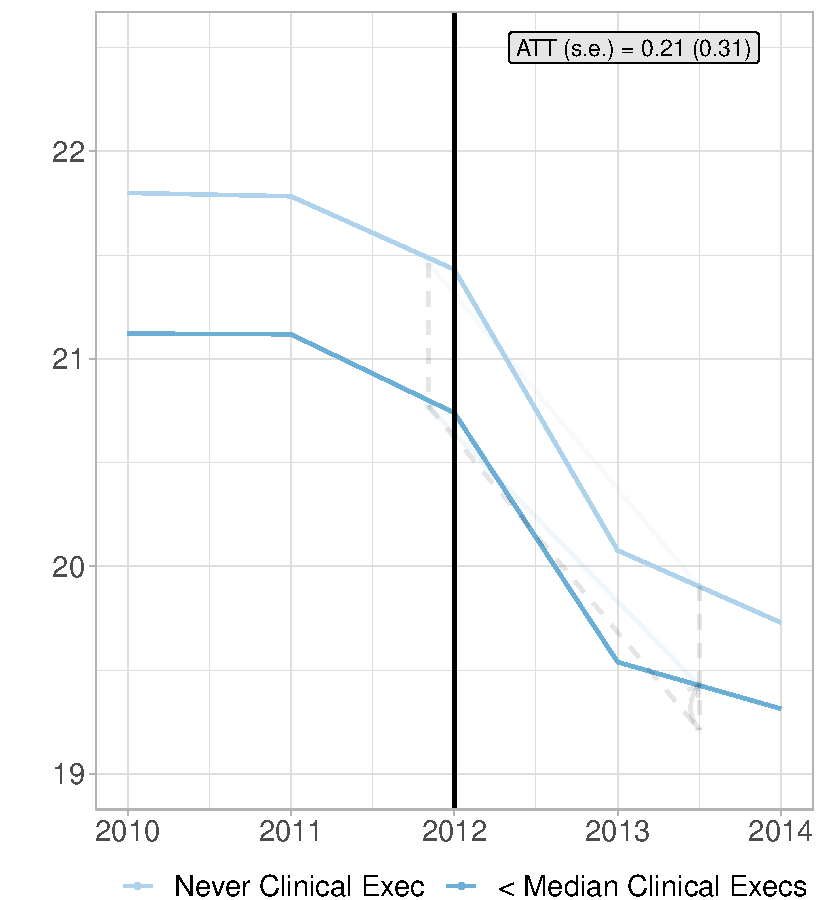
\includegraphics[width=.8\textwidth]{Objects/cont_belowmedread_md_nomd_synth_graph.pdf}
    \column{0.5\textwidth}
        \centering
        above median
        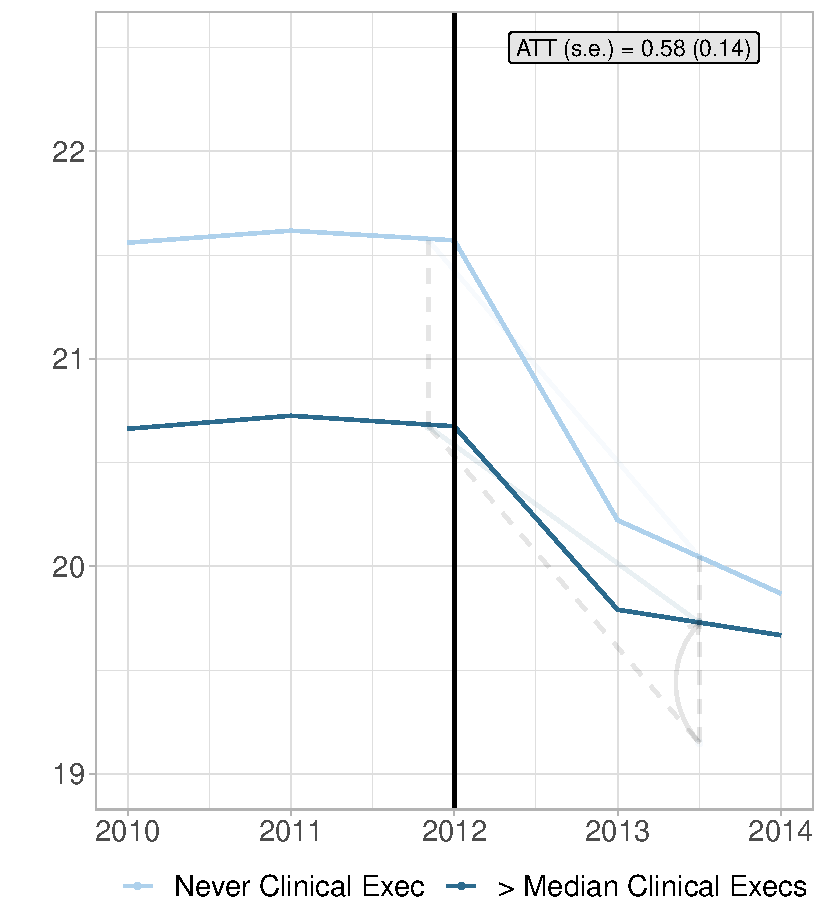
\includegraphics[width=.8\textwidth]{Objects/cont_abovemedread_md_nomd_synth_graph.pdf}
    \end{columns}
    \btVFill

    \hyperlink{main:readrates}{\beamerreturnbutton{main results}}
\end{frame}

\begin{frame}{Intensive Margin, Mortality}
    \begin{columns}
    \column{0.5\textwidth}
        \centering
        below median
        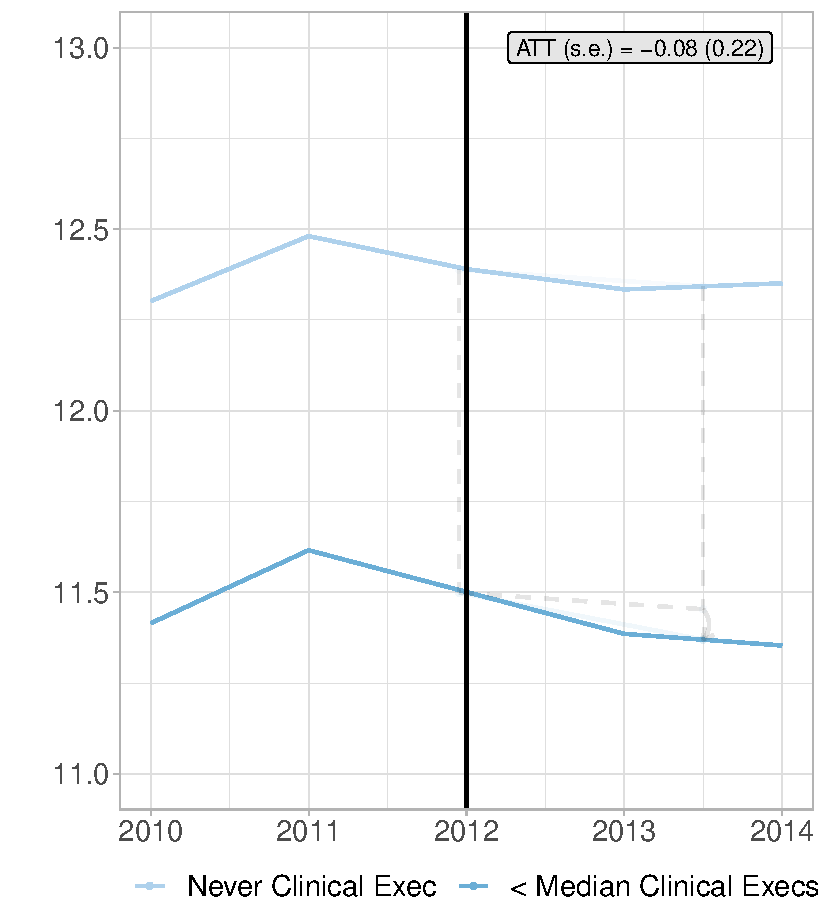
\includegraphics[width=.8\textwidth]{Objects/cont_belowmedmort_md_nomd_synth_graph.pdf}
    \column{0.5\textwidth}
        \centering
        above median
        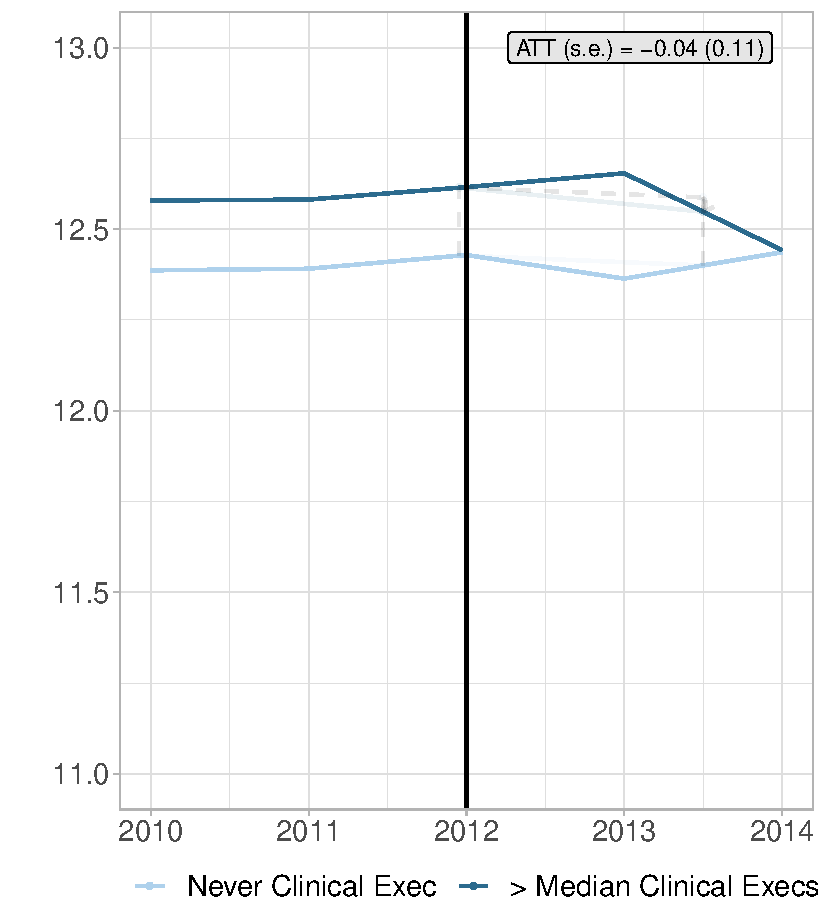
\includegraphics[width=.8\textwidth]{Objects/cont_abovemedmort_md_nomd_synth_graph.pdf}
    \end{columns}
    \btVFill

    \hyperlink{main:readrates}{\beamerreturnbutton{main results}}
\end{frame}

\begin{frame}{Due to patient selection practices?}\label{cmi}
\begin{center}
    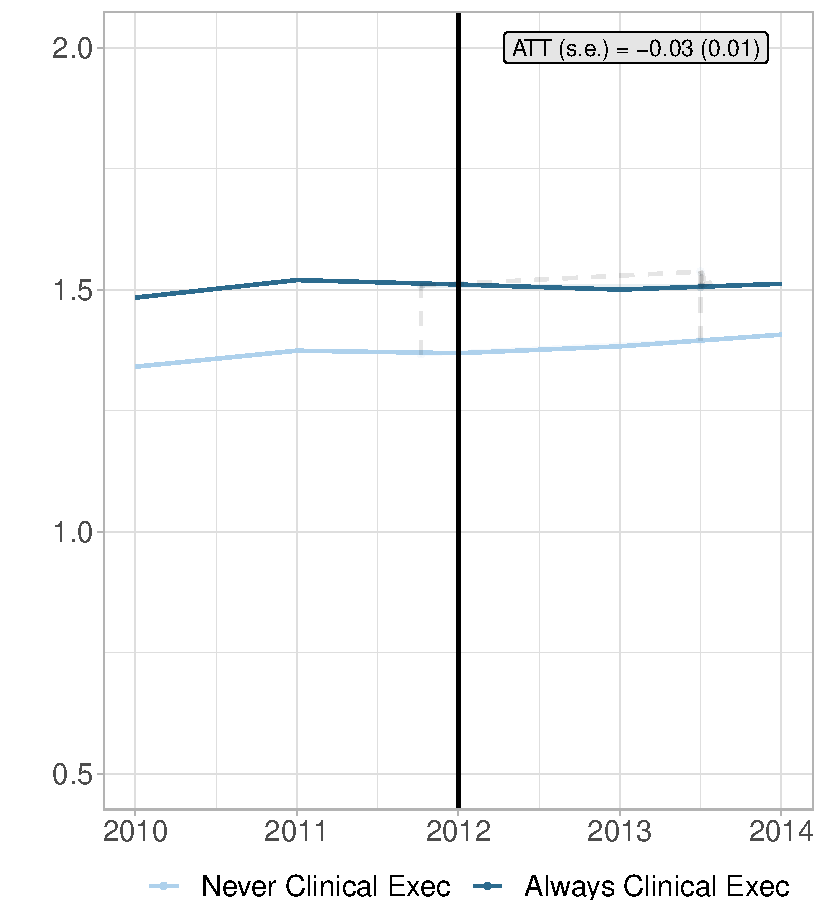
\includegraphics[width=.4\textwidth]{Objects/cmi_md_nomd_synth_graph.pdf}
\end{center}

\btVFill

\hyperlink{main:readrates}{\beamerreturnbutton{main results}}
    
\end{frame}

\begin{frame}{Results of other specifications}\label{specifications}
    \begin{table}[ht!]
\centering
\begin{tabular}[t]{lcccccl}
\toprule
\multicolumn{1}{c}{} & \multicolumn{3}{c}{Readmission Rate} & \multicolumn{3}{c}{Mortality Rate} \\
\cmidrule(l{3pt}r{3pt}){2-4} \cmidrule(l{3pt}r{3pt}){5-7}
\multicolumn{1}{c}{ } & \multicolumn{1}{c}{TWFE} & \multicolumn{1}{c}{Matched} & \multicolumn{1}{c}{SC} & \multicolumn{1}{c}{TWFE} & \multicolumn{1}{c}{Matched} & \multicolumn{1}{c}{SC} \\
\cmidrule(l{3pt}r{3pt}){2-2} \cmidrule(l{3pt}r{3pt}){3-3} \cmidrule(l{3pt}r{3pt}){4-4} \cmidrule(l{3pt}r{3pt}){5-5} \cmidrule(l{3pt}r{3pt}){6-6} \cmidrule(l{3pt}r{3pt}){7-7}
 & (1) & (2) & (3) & (4) & (5) & (6)\\
\midrule
Ever Clinical Exec x Post 2012 & 0.42$^{**}$ & 0.65$^{*}$ & 0.25 & 0.11 & 0.03 & 0.06\\
 & (0.15) & (0.3) & (0.14) & (0.15) & (0.4) & (0.12)\\
 &  &  &  &  &  & \\
Hospital FE & $\checkmark$ & $\checkmark$ & $\checkmark$ & $\checkmark$ & $\checkmark$ & $\checkmark$\\
Year FE & $\checkmark$ & $\checkmark$ & $\checkmark$ & $\checkmark$ & $\checkmark$ & $\checkmark$\\
\addlinespace
Observations & 2,387 & 1,025 & 1,640 & 2,381 & 1,023 & 1,640\\
\bottomrule
\end{tabular}
\end{table}

\btVFill

\hyperlink{main:readrates}{\beamerreturnbutton{main results}}
\end{frame}

\begin{frame}{Results by Specialty}\label{specialty}
\begin{center}
    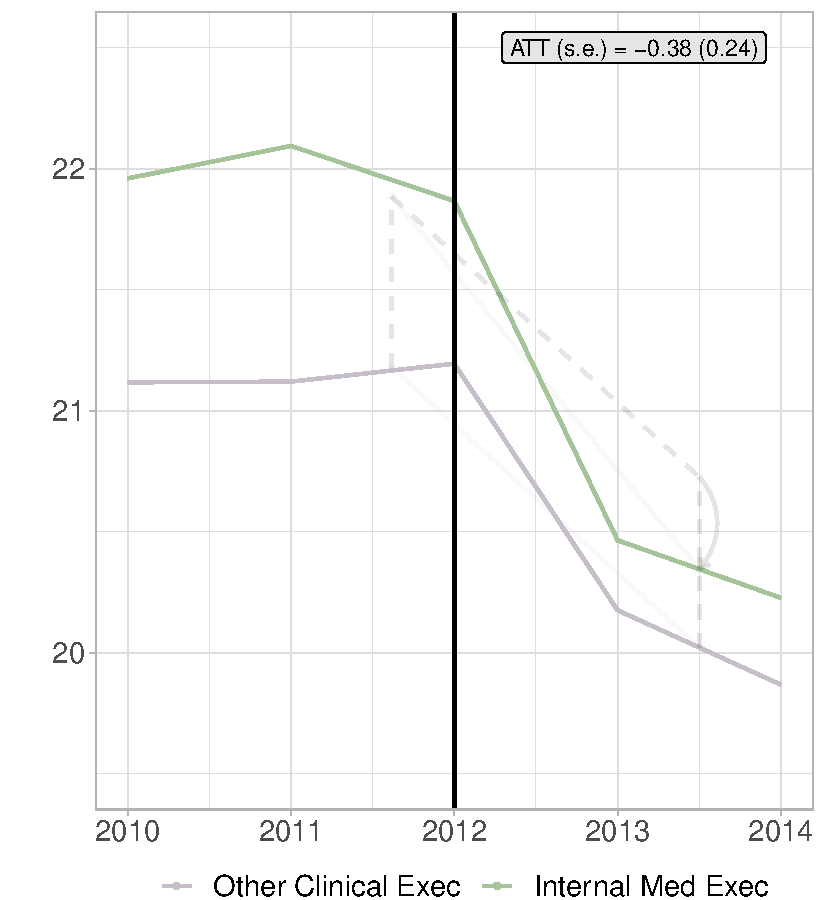
\includegraphics[width=.4\textwidth]{Objects/read_specialty_synth_graph.pdf}
\end{center}

    \btVFill

\hyperlink{main:readrates}{\beamerreturnbutton{main results}}
\end{frame}

\end{document}

